Large language models (LLMs) are trained to absorb the myriad of patterns that are woven into the structure of language. They not only exhibit various out-of-the-box capabilities such as generating chains of reasoning \cite{wei2022chain,kojima2022large}, solving logic problems \cite{suzgun2022challenging,creswell2022selection}, and completing math puzzles \cite{lewkowycz2022solving}, but also have been applied in robotics where they can serve as high-level planners for instruction following tasks \cite{ahn2022can, huang2022language, xie2023translating, ding2023task,liu2023llm+,zelikman2023parsel, lin2023text2motion}, synthesize programs representing robot policies \cite{liang2022code,singh2023progprompt}, design reward functions~\cite{kwon2023reward,hu2023language}, and generalize user preferences \cite{wu2023tidybot}. These settings rely on few-shot in-context examples in text prompts that specify the domain and input-output format for their tasks \cite{liu2021makes,zhao2021calibrate}, and remain highly semantic in their inputs and outputs.

\begin{wrapfigure}{r}{0.245\textwidth}
    \vspace{-1.3em}
    \centering
    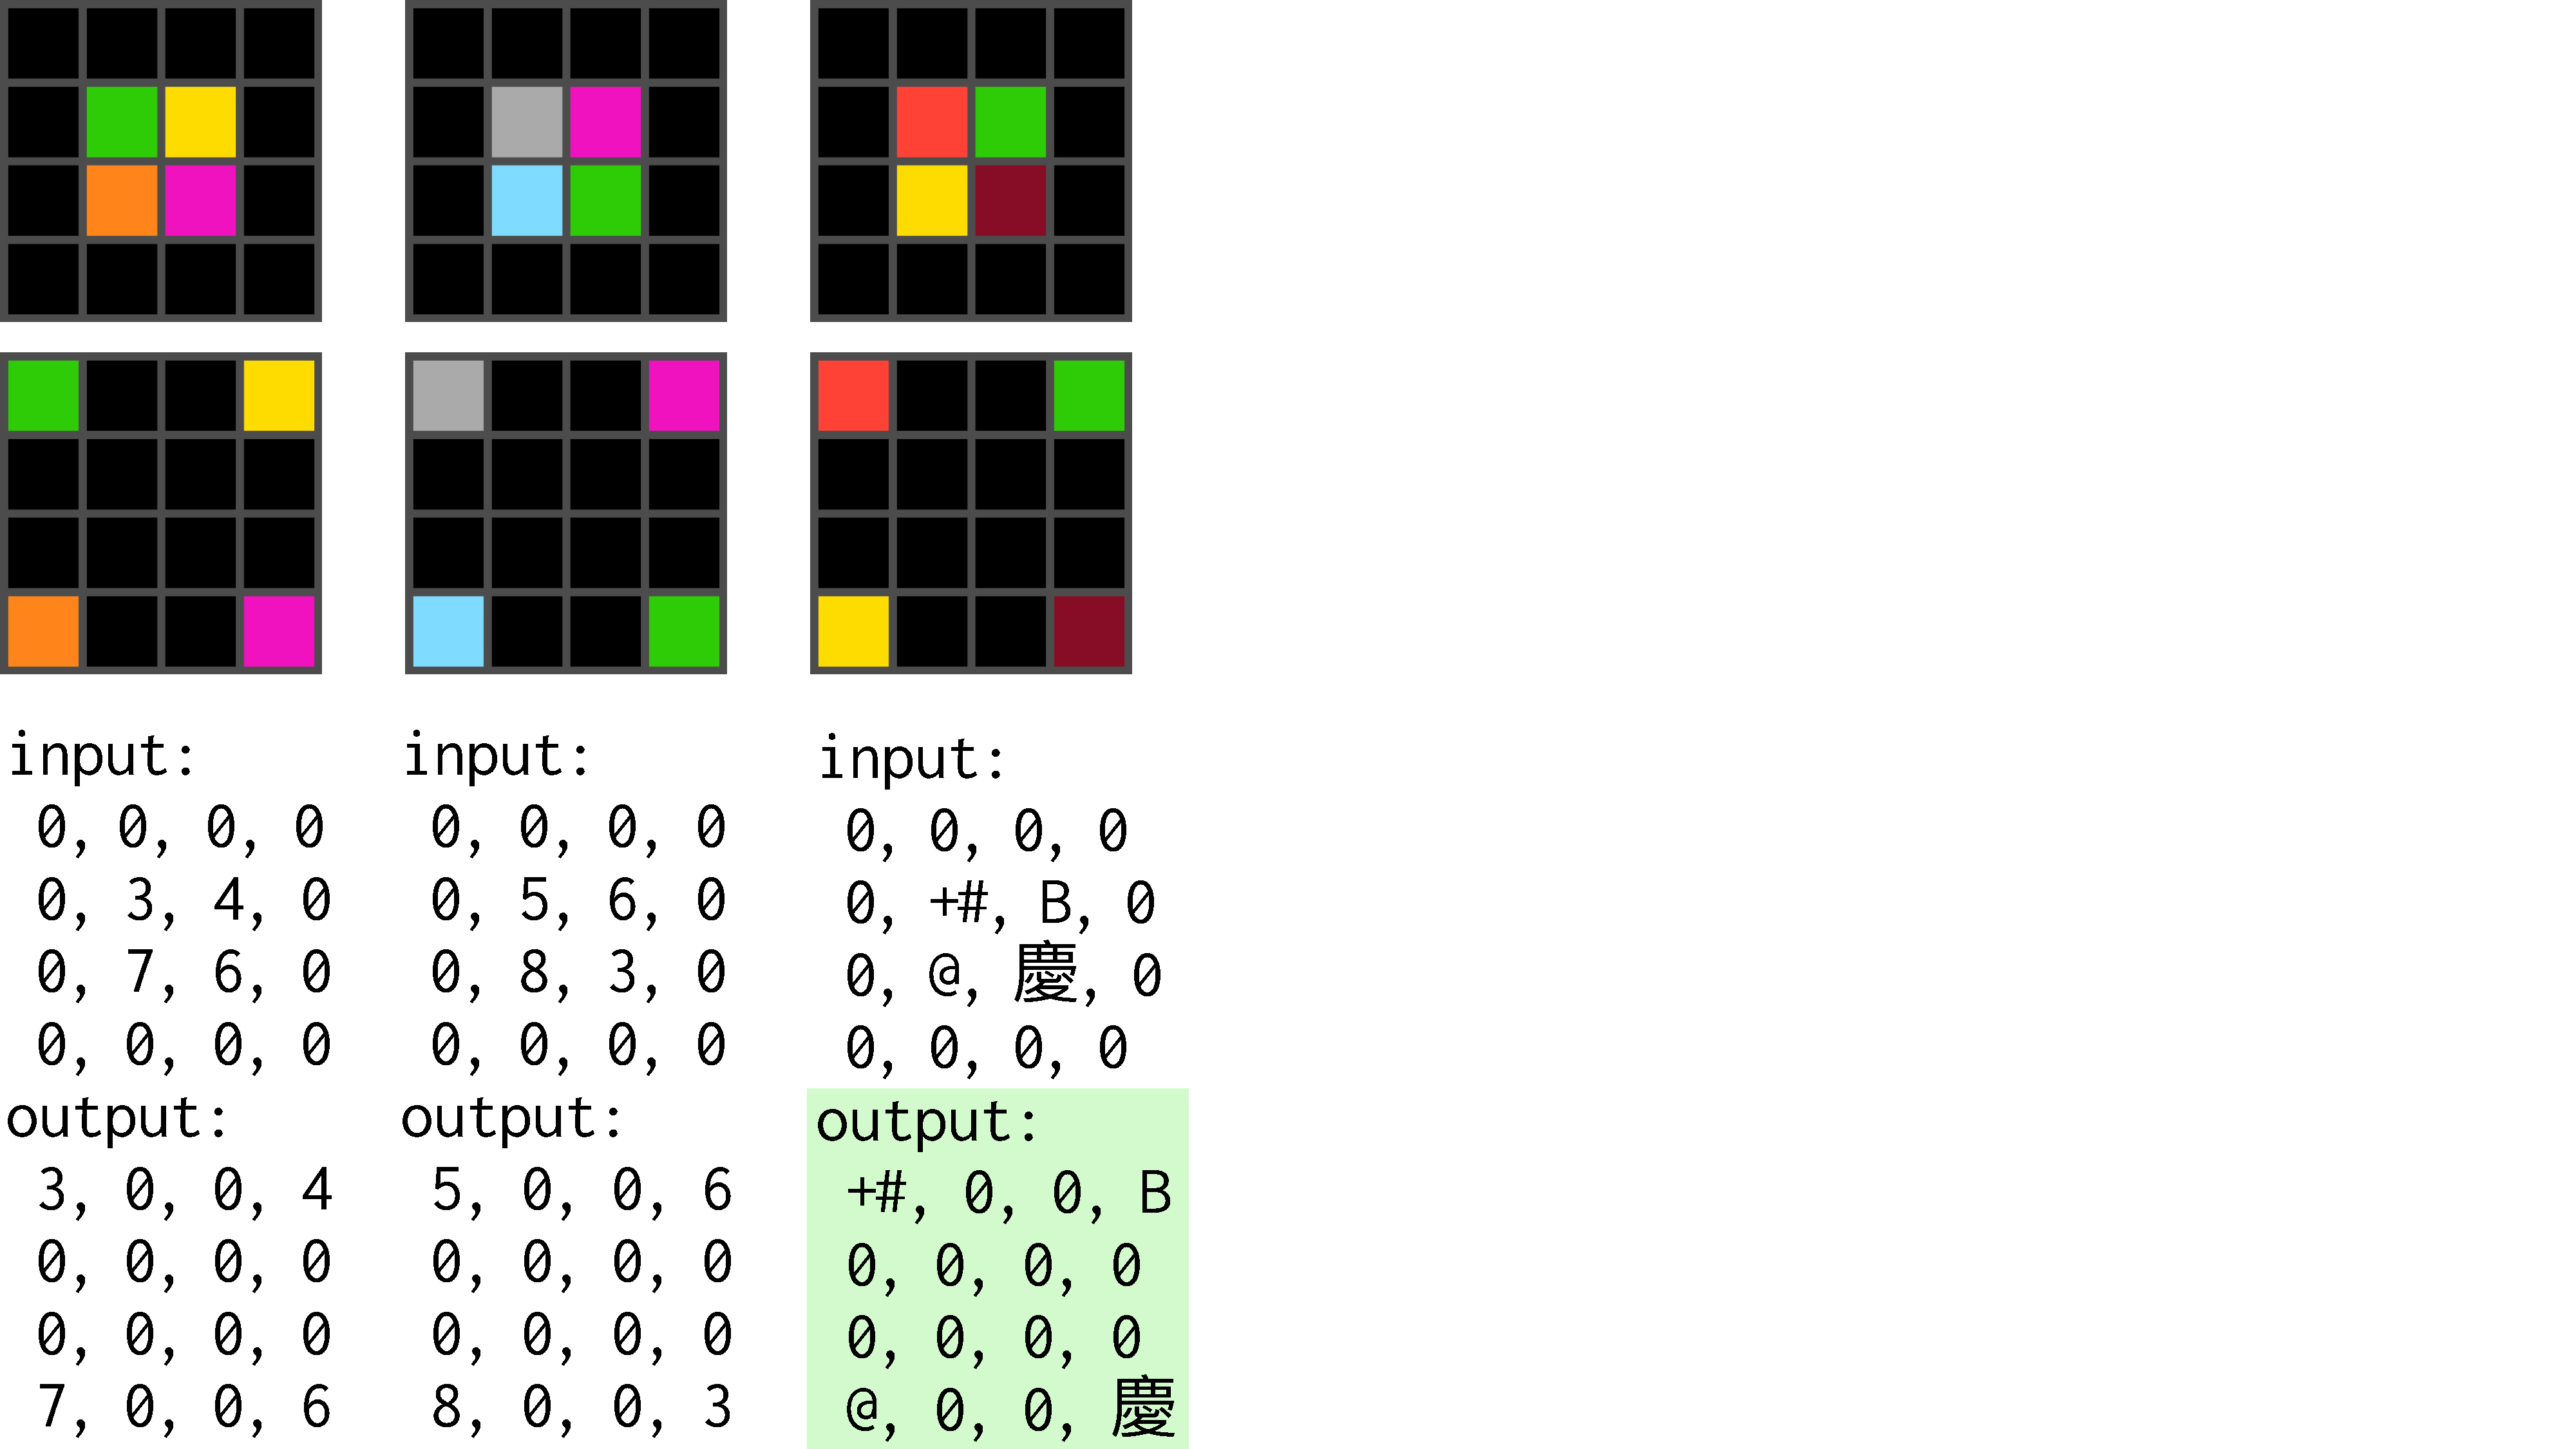
\includegraphics[width=\linewidth]{figures/arc-teaser-v3.pdf}
    \caption{
    \small
    LLMs out-of-the-box can complete ({\setlength{\fboxsep}{1pt}\colorbox{highlight}{highlighted}}) complex ARC patterns \cite{chollet2019measure} expressed in arbitrary tokens. 
    \vspace{-2.3em}
    }
    \label{fig:arc-teaser}
    \vspace{-0.7em}
\end{wrapfigure}

A key observation of our work---and perhaps contrary to the predominant intuition---is that an LLM's ability to represent, manipulate, and extrapolate \textit{more abstract, nonlinguistic} patterns may allow them to serve as basic versions of \textit{general pattern machines}. To illustrate this idea, consider the Abstraction and Reasoning Corpus \cite{chollet2019measure}, a general AI benchmark that contains collections of 2D grids with patterns that evoke abstract concepts (\eg infilling, counting, and rotating shapes). Each problem provides a small number of input-output examples, followed by test input(s) for which the objective is to predict the corresponding output. Most methods (based on program synthesis) are manually engineered with domain-specific languages \cite{ferre2021first,xu2022graphs,ainooson2023approach,alford2021neurosymbolic} or evaluated on simplified extensions or subsets of the benchmark \cite{assouel2022object,moskvichev2023conceptarc,kolev2020neural}. End-to-end machine learning methods only solve a handful of test problems \cite{paparaju2020arc}; however, our experiments indicate that LLMs in-context prompted in the style of ASCII art (see~\cref{fig:arc-teaser}) can correctly predict solutions for up to 85 (out of 800) problems---exceeding some existing recent systems \cite{ferre2021first,xu2022graphs,alford2021neurosymbolic}, without additional model training or fine-tuning. Surprisingly, we find this extends beyond ASCII numbers, and that when they are replaced with a mapping to \textit{randomly sampled tokens} in the vocabulary, LLMs can still generate some valid solutions. These results suggest an intriguing insight: that LLMs may exhibit more general capabilities of representing and extrapolating symbolic patterns, invariant to the specific tokens involved.
This is in-line with---and complementary to---recent observations that using random or abstract label mappings for in-context classification retains some performance compared to ground-truth labels \cite{min2022rethinking, pan2023context}.
We hypothesize that the capabilities that drive pattern reasoning on the ARC may allow general pattern manipulation at various levels of abstraction useful for robotics and sequential decision making \cite{lu2021pretrained,reid2022can}, wherein a diverse array of problems involve patterns that may be difficult to reason about precisely in words. For example, a procedure for spatially rearranging tabletop objects could be represented using arbitrary tokens (see \cref{fig:teaser}). As another example, optimizing a trajectory with respect to a reward function can be framed as extrapolating a sequence consisting of state and action tokens with increasing returns.

\begin{figure}[t]
    \centering
    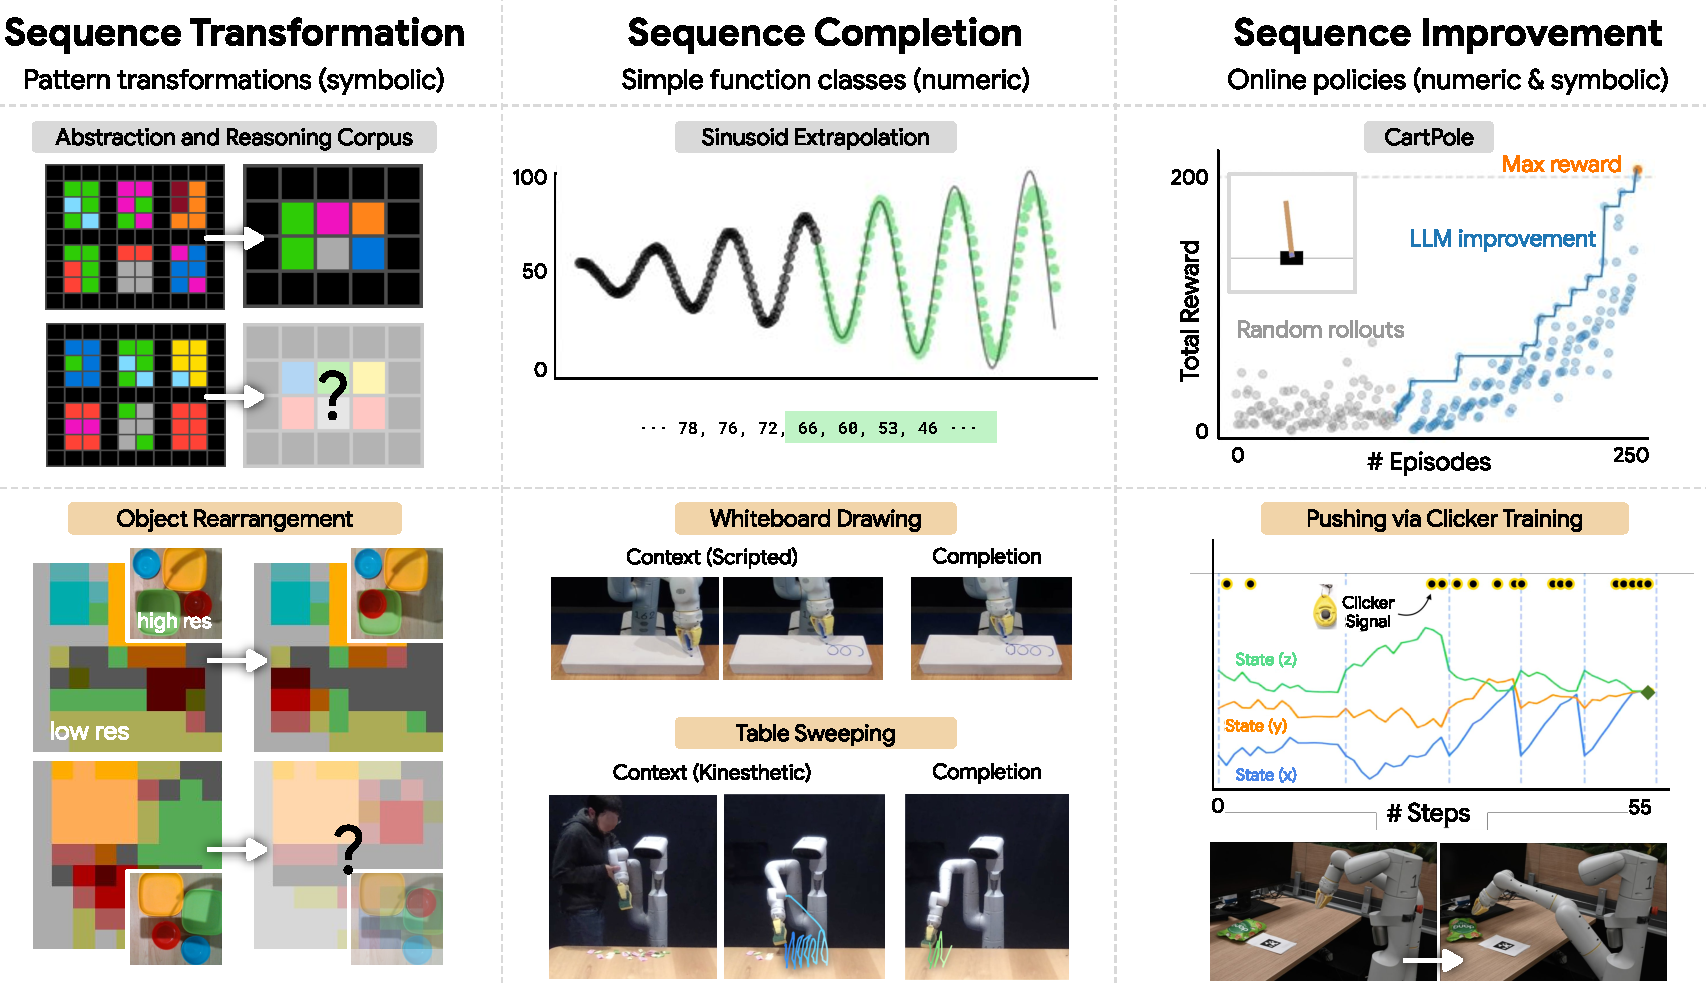
\includegraphics[width=\textwidth]{figures/pattern-machines-teaser-v7.pdf}
    \caption{\small{Pre-trained LLMs out-of-the-box may serve as basic versions of \textit{general pattern machines} that can recognize and complete sequences of numeric or arbitrary (symbolic) tokens expressing abstract problems in robotics and sequential decision-making. Experiments show that to an extent, LLMs can in-context learn (i) sequence transformations (\eg to reason over spatial rearrangements of symbols, for dynamics modeling and next state prediction on downsampled images), (ii) completion of simple functions (\eg to extrapolate kinesthetic demonstrations), or (iii) meta-patterns to improve return-conditioned policies (\eg to discover oscillatory behaviors to stabilize a CartPole).
    \vspace{-2.3em}
    }}
    \label{fig:teaser}
    \vspace{-0.5em}
\end{figure}

Orthogonal and complementary to efforts that develop multi-task policies by pre-training on large amounts of robot data \cite{brohan2022rt}, or robotics foundation models \cite{bommasani2021opportunities} that can be fine-tuned for downstream tasks~\cite{nair2022r3m,radosavovic2023real,karamcheti2023voltron}, our goal is instead to (i) assess the zero-shot capabilities that LLMs may already contain to perform some degree of general pattern manipulation, and (ii) investigate how these abilities can be used in robotics. These capabilities are certainly \textit{not} sufficient to replace specialized algorithms; nonetheless, they are useful to characterize, and doing so may help inform priorities for training generalist models in robotics.

We assess LLMs as pattern machines categorized into three areas: sequence transformation, sequence completion, and sequence improvement (\cref{fig:teaser}). First, we show that LLMs are capable of generalizing certain sequence transformations of increasing complexity with a degree of token invariance, and posit that this can carry over to spatial reasoning capabilities in robotic tasks. Next, we assess LLMs' ability to complete patterns from simple functions (\eg sinusoids) and show this can be applied to robotic tasks like extending a wiping motion from kinesthetic demonstrations, or drawing patterns on a whiteboard. The combination of in-context sequence transformation and extrapolation further enables LLMs to do basic forms of sequence improvement. We show that providing reward-labeled trajectories as context, coupled with online interaction, can enable an LLM-based agent to learn to navigate through a small grid, discover a simple CartPole controller, and optimize simple trajectories via human-in-the-loop ``clicker'' reward training. Code, benchmarks, and videos are made available at \url{https://general-pattern-machines.github.io}.
